%===============================================================================
%               File: ch2_introduction.tex
%            Author: Juan de Monasterio
%          Created: 15 Feb 2017
%    Description: Chapter 2: Data descriptions, exploration and risk maps
%===============================================================================

\chapter{Data Description and Risk Maps}
\label{cha:descr-risk}

\section{Mobile Phone Data Sources}

Our data source is anonymized traffic information from two mobile operators, in Argentina and in Mexico. Both companies service phone calls at the national level and to a number of customers than amounts to the order of millions. Both of these provide two different CDR datasets.

For our purposes, each record is represented as a tuple $\left < i, j, t, d, l \right >$,
where user $i$ is the caller, user $j$ is the callee, $t$ is the date and time of the call,
$d$ is the direction of the call (incoming or outgoing, with respect to the mobile operator client), and $l$ is the location of the tower that routed the communication.

The dataset does not include personal information from the users, such as name or phone number. The users privacy is assured by differentiating users by their hashed ID, with encryption keys managed exclusively by the telephone company.

Data was preprocessed excluding users whose monthly cellphone use either did not surpass a minimal number of calls $\mu$ or exceeded a maximal number $M$. This ensures we leave out outlying users such as call-centers or dead phones. In both datasets, we used $\mu = 5$ and $M = 400$.

We then aggregate the call records for a five 
month period into an edge list $(n_i, n_j, w_{i,j})$ where nodes $n_i$ and $n_j$ 
represent users $i$ and $j$ respectively and $w_{i,j}$ is a boolean value
indicating whether these two users have communicated at least once within the 
five month period. This edge list will represent our mobile graph   
$\calG = \left< \calN, \calE \right> $ where $\calN$ denotes the set of nodes (users) 
and $\calE$ the set of communication links. We note that only a subset $\calN_C$ nodes in $\calN$
are clients of the mobile operator, the remaining nodes $\calN \setminus \calN_C$ are
users that communicated with users in $ \calN_C $ but themselves are not clients of
the mobile operator. 

Since geolocation information is available only for users in $\calN_C$, in the analysis we considered the graph $\calG_C = \left< \calN_C, \calE_C \right> $ of communications between clients of the operator.

% \paragraph{Argentina.} 
\paragraph{Datasets Information.}

The Argentinian dataset contains CDRs collected over a period of 5 months, from November 2011 to March 2012. The raw data logs contain, in average, more than 65 million calls per day. The minimum number of logs were registered on the 26th of January whilst the day with most calls was on the 7th of December.  The user base amounts to more than 21 million live lines of \textit{active} clients. The calls were placed through a network of 4477 geolocalized antennas. In total, data amounts to almost 10 billion calls. 
% \paragraph{Mexico.} 

The Mexican data source is an anonymized dataset from a national mobile phone operator. Data is available for every call made within a period of 24 months from January 2014 to December 2015. The raw logs contain at least 11 and at most 47 million daily calls. These were for the dates of   day for more than 8 million users that accessed the telecommunication company's (\textit{telco}) network to place the call. This means that users from other companies are logged, as long as one of the users registering the call is a client of the operator. In practice, we only considered CDRs between users in $\calN_C$ since geolocalization was only possible for this group.

Information logged for each call included the duration and timestamp of the call, the users participating in the call and the antenna id that transmitted the call to the TelCo client. 


% \subsection{Data Limitations}
\paragraph{Data Limitations.}
Although a lot of information is available in the CDR datasets, there may be limitations in their representativeness of the whole population. In each case, data is sourced from a single mobile phone operator, and no information is given on the distribution of its users, thus calls might in principle not represent correctly social interactions and movements between two given jurisdictions. Also, not all user movements will be captured by the log records. However, these limitations are offset by the huge datasets' sizes, from which we can safely assume that the amount of users observed in each set is sufficient to correlate real mobility or social links between different areas.


% Si podemos reflotemos el grafico de clustering de provincias segun comunicaciones, y repitamos para estados en Mexico.


% Procedimiento:
% Obtener la lista de antenas de GC
% Determinar la casa de los usuarios
% Determinar, para cada usuario, si se comunic\selectlanguage{ngerman}ó \selectlanguage{english}con un habitante de GC
% Determinar las agregaciones por antena
% Visualizar (agrego alfa, min_volume y zoom en regiones)


\section{ Risk Map Generation} \label{methods}

In this section we describe how the Chagas disease risk maps were built for the in Argentina and in Mexico and we give an overview of the their uses. As an overview, the risk maps will display a geographical map with all of the Telco's antennas situated on the map. And for each of the antennas, a circle will be drawn on it which will represent, graphically, the volume of usage of that antenna and the vulnerability of its users. We will expand on this last concept later.

\subsection{Home Detection}

The first step determines the antenna in which each user lives. The antenna's neighborhood will define his area of influence and with this, his risk condition associated with being inside or outside the epidemic region.

Having the granularity of the geolocated data at the antenna level, we can match each user $u \in \calN_C$ with its \textit{home antenna} $H_u$. To do so, we assume $H_u$ as the antenna in which user $u$ spends most of the time during weekday nights. This, according to our categorization of days of the week's types, corresponds to Monday through Thursday nights, from 8pm to 6am of the following day. 

This \textit{home} characterization is based on the assumption that on any given day, users will be located at home during night time. The implications of this assumption for Argentinean CDRs are explored in detail in ~\cite{sarraute2015socialevents,csaji2012exploring}. The authors explain that given the large user base, this assumption proves helpful when trying to predict migration patterns.

Given the user's $H_u$, he will be considered endemic if his inferred home antenna is located in the endemic zone $E_Z$. These tagged users be considered to be the set of \textit{residents of $E_Z$}.

In the case of Argentina, the risk area is the \textit{Gran Chaco} ecoregion, as described in Section~\ref{endemic_zone_argentina};
whereas in the case of Mexico, we used the region described in Section~ \cref{endemic_zone_mexico}.


\subsection{Detection of Vulnerable Users}

Given the set of inhabitants of the risk area, we want to find those with a high communication with residents of the endemic zone $E_Z$. To do this, we get the list of calls for each user and then determine the set of their neighbors in the social graph $\calG_C$. For each resident of the endemic zone, we tag all his neighbors as potentially vulnerable. We also tag the calls to (from) a certain antenna from (to) residents of the endemic area $E_Z$ as \textit{vulnerable calls}. With our definition, a user with at least one call from (to) the endemic area is enough to tag this user as vulnerable. 

The next step is to aggregate this data for every antenna. Given an antenna $a$, we will have:
\begin{itemize}
	\item The total number of residents $N_a$ (this is, the number of people for which that is their home antenna).
	\item The total number of residents which are vulnerable $V_a$.
	\item The total volume of outgoing calls $C_a$ from every antenna.
	\item From the outgoing calls, we extracted every call that had a user whose home is in the endemic area $E_Z$ as a receiver $VC_a$ (\textit{vulnerable calls}).
\end{itemize}

These four numbers $\left< N_a, V_a, C_a, VC_a \right>$ are the properties we extracted for each antenna in the studied country.


\subsection{Heatmap Generation}
With the collected antenna properties, we generated heatmaps to visualize the mentioned antenna indicators, overlapping these heatmaps with political maps of the region taken for study.

In them, a circle is generated for each cell, where:
%	%Generamos un c\'irculo por cada celda donde:
\begin{itemize}
	\item the \textbf{area} depends on the population living in the antenna $N_a$.
	%el \textbf{\'area} depende de la cantidad de usuarios (habitantes),
	\item the \textbf{color}, is related to the fraction ${V_a}/{N_a}$ of vulnerable users living there.
	%		%el \textbf{color} corresponde al porcentaje de usuarios vulnerables que viven en esa antena.
\end{itemize}

%
%A circle is generated for each antenna, where
%the \textbf{area} depends on the population living in the antenna $N_a$;
%and the \textbf{color} is related to the fraction ${V_a}/{N_a}$ of vulnerable users living there.

We used two filtering parameters to control which antennas are plotted.
\begin{itemize}
	\item $\beta$: The antenna is plotted if its fraction of vulnerable users is higher than $\beta$.
	\item $m_v$: The antenna is plotted if its population is bigger than $m_v$.
\end{itemize}

When displaying the maps, these parameters were helpful to identify special small antennas which were covered under the plots of other antennas. Also, they were tuned differently for different regions. For example: an antenna whose vulnerable percentage would be considered low at the national level can be locally high when zooming in at a more regional level. These filtering parameters helped us explore these cases with more detail.


\section{Resulting Observations} \label{results}

\subsection{Risk Maps for Argentina}


\begin{figure}[h!]
	
	\begin{minipage}{.495\linewidth}
		\centering
		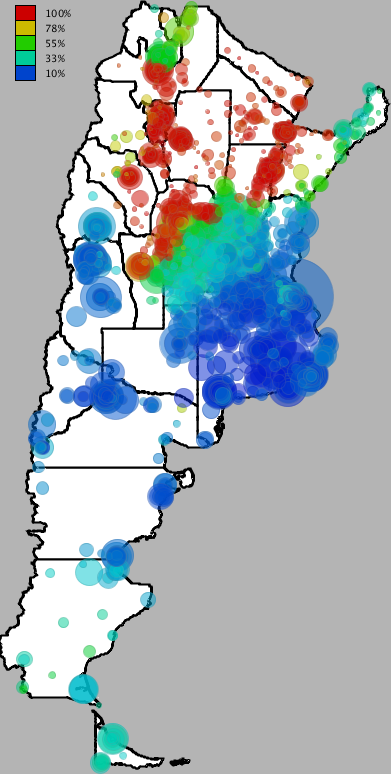
\includegraphics[width=0.90\linewidth]
		{figures/201112_hi_res_argentina_usuarios_proporcion_circulos_beta1/201112_hi_res_argentina_usuarios_proporcion_circulos_beta1}
		
		(a) $\beta = 0.01$
	\end{minipage}
	\begin{minipage}{.495\linewidth}
		\centering
		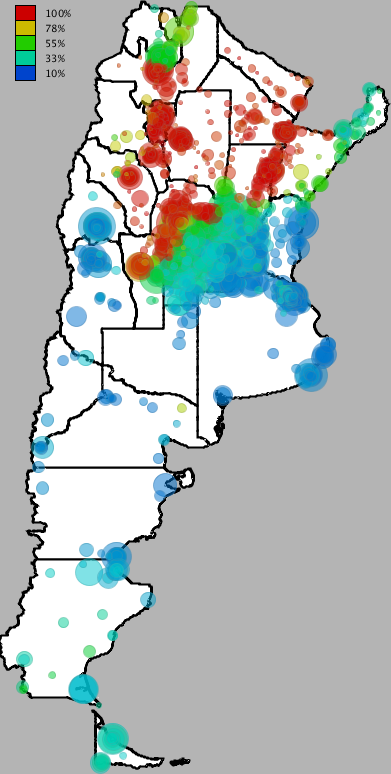
\includegraphics[width=0.90\linewidth]
		{figures/201112_hi_res_argentina_usuarios_proporcion_circulos_beta15/201112_hi_res_argentina_usuarios_proporcion_circulos_beta15}
		
		(b) $\beta = 0.15$
	\end{minipage}
	\caption{Risk map for Argentina, filtered according to $\beta$.}
	\label{fig:mapa_argentina}
\end{figure}

As a first visualization, maps were drawn using a provincial or national scale.
Advised by \textit{Mundo Sano} Foundation's experts, we then focused on areas of specific epidemic interest. 

Figure~ \cref{fig:mapa_argentina} shows the risk maps for Argentina, generated with
two values for the $\beta$ filtering parameter, and fixing $m_v = 50$ inhabitants per antenna. After filtering with $\beta = 0.15$, we see that large portions of the country harbor potentially vulnerable individuals.
Namely, Figure~ \cref{fig:mapa_argentina}(b) shows antennas where more that 15\% of the population has social ties with the endemic region $E_Z$.

Figure~ \cref{fig:cba_sfe} shows a close-up for the Cordoba and Santa Fe provinces,
where we can see a gradient from the regions closer to the endemic zone $E_Z$ to the ones further away.


\begin{figure}[p]
	\centering
	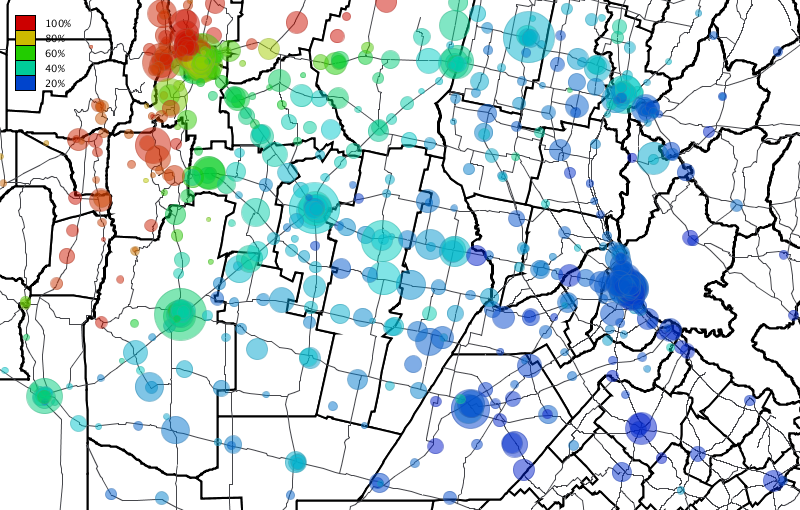
\includegraphics[width=0.95\linewidth]
	{figures/201112_hi_res_cba_sfe_usuarios_proporcion_circulos_beta15/201112_hi_res_cba_sfe_usuarios_proporcion_circulos_beta15}
	\caption{Risk map for Cordoba and Santa Fe provinces, filtered according to $\beta = 0.15$.}
	\label{fig:cba_sfe}
\end{figure}



\subsection{Detection of Vulnerable Communities}
% Mapas
% Histograma de porcentaje de vulnerabilidad por antena?
% Cambios en los colores de los mapas (aclarar que el codigo de color cambia)

As a result of inspecting the maps in Figure~ \cref{fig:mapa_argentina}, we decided to 
focus visualizations in areas whose results were unexpected to the epidemiological experts. 
These areas included the provinces of Tierra del Fuego, Chubut, Santa Cruz and Buenos Aires, with special focus on the metropolitan area of Greater Buenos Aires whose heatmap is shown in Figure~ \cref{fig:amba_map}.

In some cases, antennas stood out for having a significantly higher link to the epidemic area than the adjacent ones. Our objective here was to enhance the visualization in areas outside of Gran Chaco looking for possible host communities of migrants from the ecoregion, infered by the social links given by the CDRs. Our assumptions were that if, in average, there was a high percentage of vulnerable users in that non-epidemic antenna, this would mean that there's a high possibility of having more infected users in that community.

As a result of this visualization, high risk antennas were separately listed and manually located in political maps. This information was made available to the \textit{Mundo Sano} Foundation collaborators who used it as an aid for their campaign planning and as education for community health workers. 


\begin{figure}[p]
	\centering
	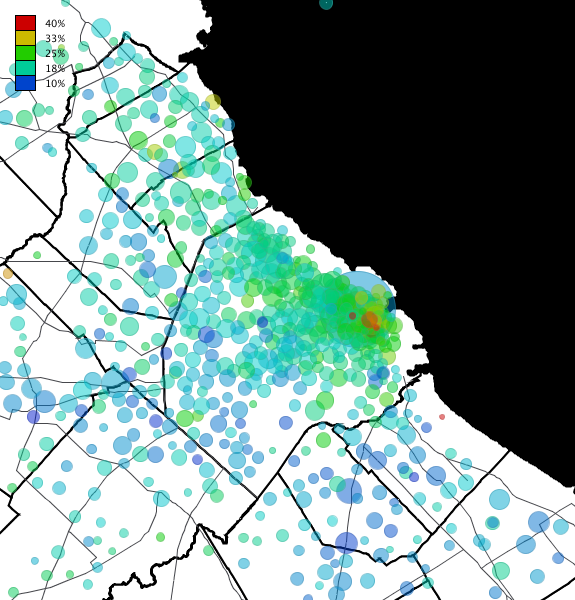
\includegraphics[width=0.75\linewidth]
	{figures/201112_hi_res_amba_usuarios_proporcion_circulos_beta2/201112_hi_res_amba_usuarios_proporcion_circulos_beta2}
	\caption{Risk map for the metropolitan area of Buenos Aires, filtered with $\beta = 0.02$.}
	\label{fig:amba_map}
\end{figure}

\begin{figure}[h!]
	\begin{center}
		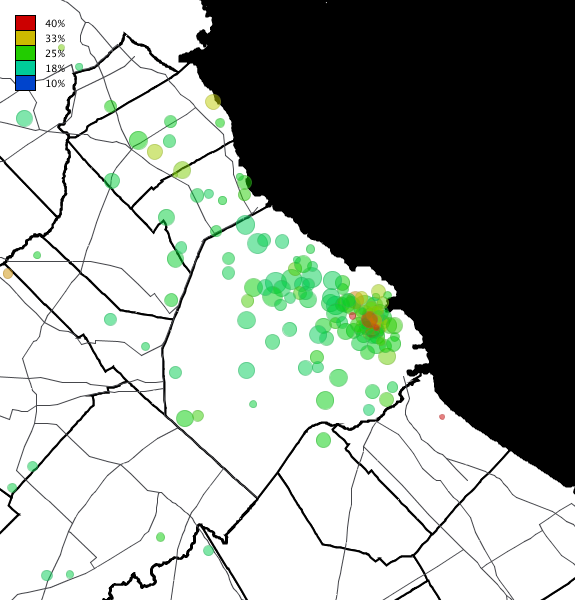
\includegraphics[width=0.35\columnwidth]{figures/201112_hi_res_amba_usuarios_proporcion_circulos_beta20/201112_hi_res_amba_usuarios_proporcion_circulos_beta20}
		\caption{Replace this text with your caption%
		}
	\end{center}
\end{figure}

This data exploration allowed us to specifically detect outlying communities in the focused regions. Some of these can be seen directly from the heatmap in Figure~ \cref{fig:amba_map}, where the towns of Avellaneda, San Isidro and Parque Patricios have been pinpointed.


\newpage

\subsection{Risk Maps for Mexico}

With the data provided by the CDRs and the endemic region defined in Section~ \cref{endemic_zone_mexico}, heatmaps were generated for Mexico using the methods described in Section~ \cref{methods}. The first generated visualizations are depicted in Figure~ \cref{fig:mapas_mexico},
which includes a map of the country of Mexico, and a zoom-in on the South region of the country.
We used $m_v = 80$ inhabitants per antenna, and a high filtering value $\beta = 0.50$, which 
means that in all the antennas shown in Figure~ \cref{fig:mapas_mexico},
more that 50\% of inhabitants have a social tie with the endemic region $E_Z$.
For space reasons, we don't provide here more specific visualizations and analysis of the regions of Mexico.

\begin{figure}[ht!]
	\begin{minipage}{.475\linewidth}
		\centering
		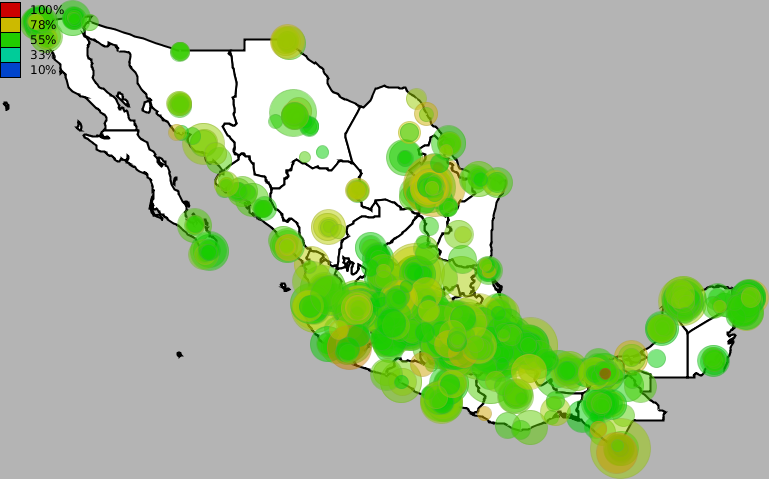
\includegraphics[width=0.95\columnwidth,height=3.2cm,keepaspectratio]
		{figures/mexico_usuarios_volumen_circulos_allday_beta--50_min_volume--80_mexico_/mexico_usuarios_volumen_circulos_allday_beta--50_min_volume--80_mexico_}
		
		(a) National map, $\beta = 0.50$
	\end{minipage}
	\begin{minipage}{.520\linewidth}
		\centering
		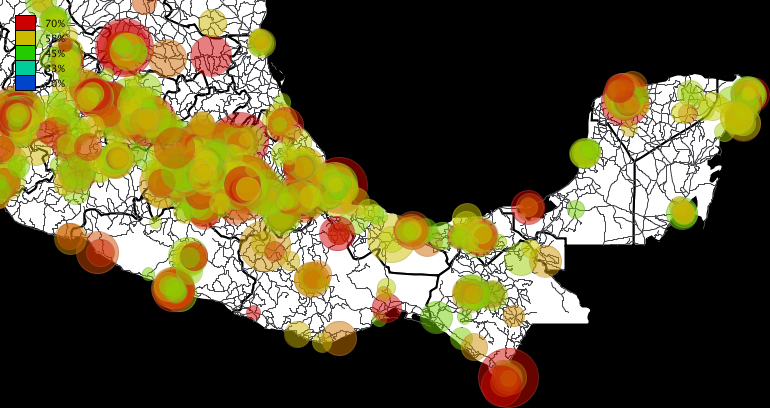
\includegraphics[width=0.95\columnwidth,height=3.2cm,keepaspectratio]
		{figures/sur_usuarios_volumen_circulos_allday_beta--50_min_volume--80_mexico_/sur_usuarios_volumen_circulos_allday_beta--50_min_volume--80_mexico_}
		
		(b) South region of Mexico, $\beta = 0.50$
	\end{minipage}
	
	\begin{minipage}{.32\linewidth}
		\centering
		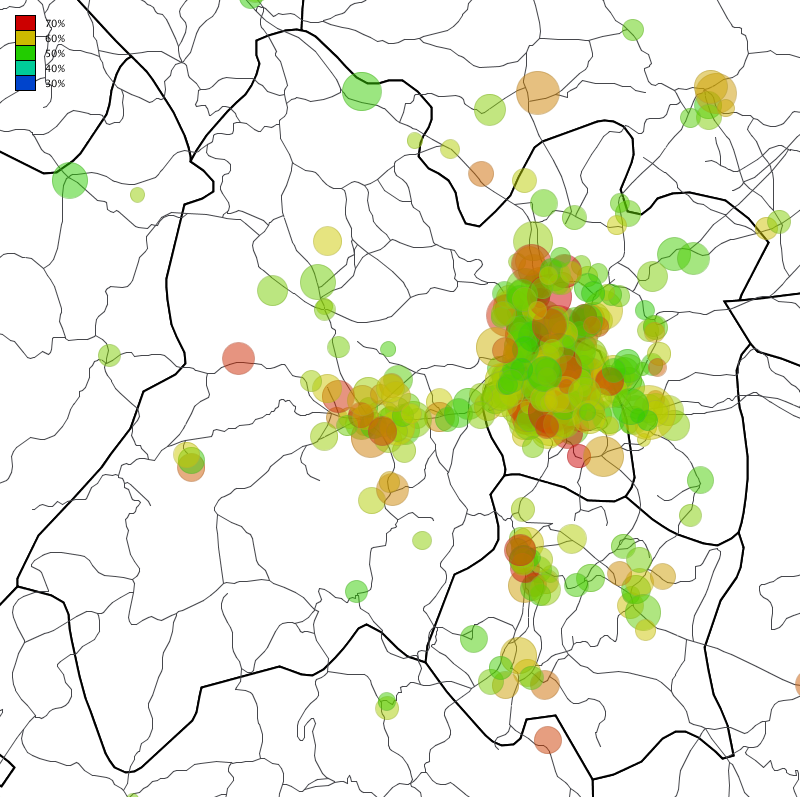
\includegraphics[width=0.90\columnwidth]
		{figures/estado_mexico_usuarios_volumen_circulos_allday_beta--50_min_volume--80_mexico_/estado_mexico_usuarios_volumen_circulos_allday_beta--50_min_volume--80_mexico_}
		
		(c) State of Mexico, $\beta = 0.50$
	\end{minipage}
	\caption{Risk maps for Mexico}
	\label{fig:mapas_mexico}
\end{figure}


\newpage

\section{Features in the Data}

The quality of any classification task with this dataset relies on the ability to characterize the users and their communication patterns, in ways that are as differentiating as possible for the task at hand. 
In general, the features constructed reflect calling and mobility patterns,
segmented by different time periods during the week, and tagging whether the actions or subjects are `endemic'. 
The training data runs from August 2015 to December 2015 (period $T_1$) and all CDRs are processed to extract features by user and by link. 

Each week is divided into time periods: 
\begin{definition} \label{def:week-periods}
	
	(i) the period \textit{weekday} is from Monday to Friday, on working hours (from 8hs to 20hs); (ii) \textit{weeknight} is from Monday to Friday, between 20hs and 8hs of the following day;
	and (iii) \textit{weekend} is Saturday and Sunday.	
\end{definition}


The model consists of the following features, which can be classified in 4 categories:
% The data is aggregated by user and by link.0


\subsection{Used and home antennas.}\label{homeantenna}

For each user $u \in \calN_C$, we register the top ten most used antennas, during each month of the training period,
together with the number of calls made through each antenna. We tag all users having their home antenna in the epidemic region as \textit{EPIDEMIC}. 

In our dataset user antennas are order with $0$ being the most used antenna and $9$ the least. We fill with null values for those users for which we don't have ten used antennas and discard users that have no calls on weeknights\footnote{This is because we wouldn't be able to detect $H_u$.}.
%Which 10 antennas does a user use most during each month of the training month interval? 
%
%How many calls have been made through each antenna? 
%
%Sort antennas with 0 being the most used and 10 the least used. Fill with nulls when less than 10 antennas were used.
We also register the most used antennas considering only calls made during the \textit{weeknight} period, as defined in \cref{def:week-periods}. % that is from Monday to Friday excluding the working hours (from 8hs to 20hs)\label{WEEKNIGHT}.
% Log counts as well.

A user's home antenna is defined by the most used antenna. For our algorithms we considered two versions, the most used antenna in all of $T_0$., and the most used antenna during the \textit{week night} for 5 months. 
With this, users were tagged as `endemic' if their home antenna is in the endemic zone $E_Z$ and `exposed' if any of the ten antennas logged is in the risk area.


\subsection{Mobility diameter.}

The user's logged antennas define a convex hull in space and the radius of the hull is taken to be as the mobility diameter. This length is representative of the area of influence of that individual, a feature expected to be correlated with long-term migrations.

We register the mobility diameter of each user, as the diameter of the convex hull defined by his top 10 used antennas. Again, we generate two values, considering (i) all antennas and (ii) only the antennas used during the \textit{weeknight}.



\subsection{Graph data and communications.}

We look at the social graph $\calG_C$ built from the CDRs, and the communications between nodes in $\calN_C$.

For each edge $\left< n_i, n_j \right> \in \calE_C$, we dive into each of their interactions, segmenting call data with different criteria. For %\textbf{each} 
each month and each pair of users $\left< i,j \right>$, we gather the tuple $\left< time_{ij}, calls_{ij}, dir, period \right>$ where $time$ is the sum of all calls (in seconds), $calls$ is the number of calls exchanged, $dir$ is a boolean variable indicating whether the calls were incoming or outgoing (from user $i$'s point of view) and $period$ corresponds to a segmentation of the week into the periods \textit{weekday}, \textit{weeknight}, and \textit{weekend}.


In this sense, two users $u_i, u_j \in \calN_C, u_i \neq uj$ are \textbf{neighbors} in the social graph if $time_{ij} > 0$.

%\begin{description}
%     \item [Neighbors.] From the social graph built from the CDRs we extracted the total count of neighbors in the communication graph and the total count of epidemic neighbors. 
%      \item [Calls.] For each month, the total time and count of monthly calls made during is aggregated per user. This information is also segmented according to the hour of the day that the calls were made and whether they were made during the weekends. Special care was taken with calls placed to and from vulnerable users and aggregated accordingly.
%\end{description}

%if we find that user $j$ is epidemic. This may be translated as the edge is vulnerable if one of both users is epidemic.

Since the samples in our dataset are users, we have to aggregate all these variables, by grouping interactions at the user level. The combination of different variables amounts to a total of 130 features per user.

To illustrate the point, we show a small example of how two calling features could look like. Groupings and filters are applied only on the user's calls:

\begin{table}[ht]
	\caption{Graph Data Features Example}
	\label{tab:data_example}
	\centering
	\begin{tabular} {|p{1.5cm}|p{1.5cm}|p{2cm}|p{1.5cm}|p{2cm}|p{1.5cm}|p{1cm}}
		%{l r r r r r r }
		\toprule
		Feature name & Call/Time & Time Period & Direction & Endemicity & Month\\
		\midrule
		Calls WeekEnd InVul08       & Count of calls & Placed on WeekEnds & Incoming calls & Edges with endemic neighbours only & August\\
		\midrule
		Time WeekNight Out12 & Sum of duration in seconds & During weekdays and on out-of-office hours & Outgoing   & No endemic filtering   & December \\
		
		\bottomrule
	\end{tabular}
\end{table}


%TimeWeekNight_OUT_12
%CallsWeekEnd_IN_12

Finally we aggregate all these variables at the user level, summing over all columns and grouping by user. 
In practice, this means grouping either by $j$ or $i$, and summing across all of the different components shown above.

We also label each edge $\left< n_i, n_j \right> \in \calE_C$ if one or both users is endemic and
ands count each user's amount of neighbors in the communication graph, as well as the endemic neighbors. This labeling defines user $i$ as \textit{vulnerable} whenever he has any edge with another user $j$ who lives in the endemic region $E_Z$. 

%% el vulnerable NO es el edge, sino que es el usuario . 
%La idea es, parate en el nodo i, hace algun filtro - o ninguno - de weeknight, in/out, weekend, mes, etc. y ahora decime
%% if $\exists j$ such that edge $ij$ existe en el grafo de llamados (con el filtro que hayamos usado en ese momento puesto).
%%

%Additionally, for each user, we extract the total 

